\section{Results}

\subsection{Complete benchmark comparison}

Tables~\ref{tab:benchmark-aupr} and \ref{tab:benchmark-auc} report test performance from the complete frozen-fold benchmark. The accompanying source-data CSV records every seed--fold value and the paired-comparison file contains raw and Benjamini--Hochberg-adjusted Wilcoxon $p$-values.

\begin{figure*}[t]
\centering
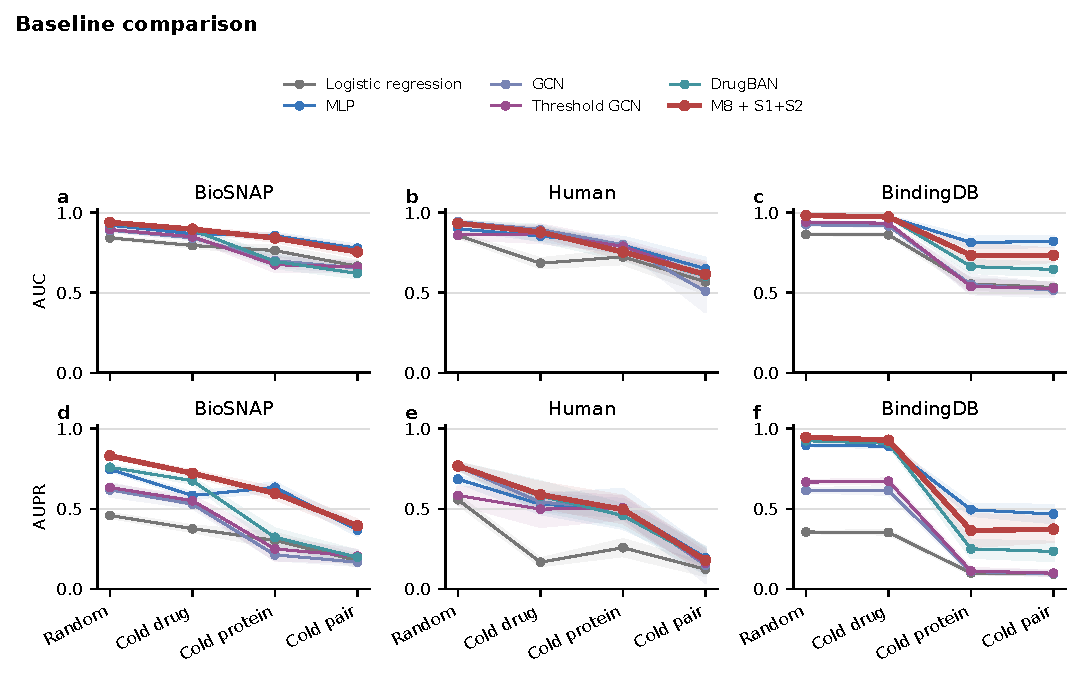
\includegraphics[width=\textwidth]{figures/figure_2_baselines.pdf}
\caption{Comparison of feature-only, graph-based, bilinear-attention and full S1/S2 models across the four fixed split scenarios. Each point is the mean of 15 seed--fold evaluations and the shaded band denotes the sample standard deviation.}
\label{fig:baseline-comparison}
\end{figure*}

Across the 12 prespecified dataset--split conditions, ArnoldiGCL-S1/S2 had the highest mean AUPR among the principal baselines in 7/12 conditions. The conditions without the highest mean AUPR were BioSNAP Cold protein, Human Cold protein, Human Cold pair, BindingDB Cold protein, BindingDB Cold pair.

\begin{table*}[t]
\centering
\scriptsize
\resizebox{\textwidth}{!}{%
\begin{tabular}{llcccccc}
\toprule
Dataset & Split & Logistic regression & MLP & GCN & Threshold GCN & DrugBAN & M8 + S1+S2 \\
\midrule
BioSNAP & Random & 0.458 $\pm$ 0.012 & 0.746 $\pm$ 0.008 & 0.618 $\pm$ 0.039 & 0.633 $\pm$ 0.016 & 0.759 $\pm$ 0.010 & 0.831 $\pm$ 0.007 \\
BioSNAP & Cold drug & 0.376 $\pm$ 0.019 & 0.583 $\pm$ 0.017 & 0.529 $\pm$ 0.022 & 0.551 $\pm$ 0.025 & 0.675 $\pm$ 0.017 & 0.722 $\pm$ 0.015 \\
BioSNAP & Cold protein & 0.303 $\pm$ 0.044 & 0.634 $\pm$ 0.030 & 0.212 $\pm$ 0.031 & 0.250 $\pm$ 0.070 & 0.322 $\pm$ 0.052 & 0.597 $\pm$ 0.034 \\
BioSNAP & Cold pair & 0.177 $\pm$ 0.034 & 0.367 $\pm$ 0.034 & 0.166 $\pm$ 0.021 & 0.203 $\pm$ 0.037 & 0.197 $\pm$ 0.039 & 0.394 $\pm$ 0.036 \\
\midrule
Human & Random & 0.557 $\pm$ 0.027 & 0.685 $\pm$ 0.019 & 0.765 $\pm$ 0.018 & 0.584 $\pm$ 0.054 & 0.766 $\pm$ 0.021 & 0.768 $\pm$ 0.018 \\
Human & Cold drug & 0.166 $\pm$ 0.022 & 0.529 $\pm$ 0.059 & 0.541 $\pm$ 0.052 & 0.498 $\pm$ 0.109 & 0.579 $\pm$ 0.091 & 0.588 $\pm$ 0.075 \\
Human & Cold protein & 0.257 $\pm$ 0.050 & 0.500 $\pm$ 0.123 & 0.503 $\pm$ 0.055 & 0.506 $\pm$ 0.070 & 0.458 $\pm$ 0.067 & 0.496 $\pm$ 0.083 \\
Human & Cold pair & 0.122 $\pm$ 0.039 & 0.195 $\pm$ 0.052 & 0.149 $\pm$ 0.107 & 0.160 $\pm$ 0.062 & 0.177 $\pm$ 0.084 & 0.178 $\pm$ 0.065 \\
\midrule
BindingDB & Random & 0.355 $\pm$ 0.004 & 0.897 $\pm$ 0.003 & 0.615 $\pm$ 0.010 & 0.667 $\pm$ 0.010 & 0.925 $\pm$ 0.004 & 0.947 $\pm$ 0.003 \\
BindingDB & Cold drug & 0.352 $\pm$ 0.011 & 0.891 $\pm$ 0.010 & 0.614 $\pm$ 0.024 & 0.673 $\pm$ 0.014 & 0.909 $\pm$ 0.010 & 0.928 $\pm$ 0.007 \\
BindingDB & Cold protein & 0.099 $\pm$ 0.009 & 0.494 $\pm$ 0.036 & 0.108 $\pm$ 0.010 & 0.111 $\pm$ 0.016 & 0.250 $\pm$ 0.053 & 0.364 $\pm$ 0.100 \\
BindingDB & Cold pair & 0.093 $\pm$ 0.006 & 0.467 $\pm$ 0.054 & 0.095 $\pm$ 0.015 & 0.098 $\pm$ 0.013 & 0.234 $\pm$ 0.058 & 0.373 $\pm$ 0.077 \\
\bottomrule
\end{tabular}%
}
\caption{Test AUPR for the principal baseline comparison. Values are mean $\pm$ sample standard deviation across 15 fixed seed--fold evaluations.}
\label{tab:benchmark-aupr}
\end{table*}

\begin{table*}[t]
\centering
\scriptsize
\resizebox{\textwidth}{!}{%
\begin{tabular}{llcccccc}
\toprule
Dataset & Split & Logistic regression & MLP & GCN & Threshold GCN & DrugBAN & M8 + S1+S2 \\
\midrule
BioSNAP & Random & 0.842 $\pm$ 0.005 & 0.922 $\pm$ 0.005 & 0.890 $\pm$ 0.008 & 0.894 $\pm$ 0.006 & 0.930 $\pm$ 0.003 & 0.939 $\pm$ 0.004 \\
BioSNAP & Cold drug & 0.795 $\pm$ 0.011 & 0.868 $\pm$ 0.008 & 0.842 $\pm$ 0.013 & 0.850 $\pm$ 0.013 & 0.892 $\pm$ 0.008 & 0.897 $\pm$ 0.008 \\
BioSNAP & Cold protein & 0.763 $\pm$ 0.028 & 0.856 $\pm$ 0.015 & 0.700 $\pm$ 0.036 & 0.675 $\pm$ 0.043 & 0.696 $\pm$ 0.040 & 0.841 $\pm$ 0.022 \\
BioSNAP & Cold pair & 0.665 $\pm$ 0.032 & 0.777 $\pm$ 0.021 & 0.654 $\pm$ 0.027 & 0.661 $\pm$ 0.032 & 0.620 $\pm$ 0.027 & 0.755 $\pm$ 0.028 \\
\midrule
Human & Random & 0.858 $\pm$ 0.012 & 0.899 $\pm$ 0.009 & 0.944 $\pm$ 0.007 & 0.860 $\pm$ 0.023 & 0.939 $\pm$ 0.008 & 0.934 $\pm$ 0.006 \\
Human & Cold drug & 0.684 $\pm$ 0.028 & 0.854 $\pm$ 0.027 & 0.894 $\pm$ 0.014 & 0.868 $\pm$ 0.056 & 0.871 $\pm$ 0.050 & 0.878 $\pm$ 0.025 \\
Human & Cold protein & 0.724 $\pm$ 0.043 & 0.796 $\pm$ 0.050 & 0.799 $\pm$ 0.018 & 0.789 $\pm$ 0.036 & 0.751 $\pm$ 0.045 & 0.755 $\pm$ 0.043 \\
Human & Cold pair & 0.569 $\pm$ 0.072 & 0.650 $\pm$ 0.067 & 0.508 $\pm$ 0.128 & 0.610 $\pm$ 0.069 & 0.604 $\pm$ 0.067 & 0.614 $\pm$ 0.077 \\
\midrule
BindingDB & Random & 0.865 $\pm$ 0.002 & 0.978 $\pm$ 0.001 & 0.924 $\pm$ 0.002 & 0.941 $\pm$ 0.002 & 0.979 $\pm$ 0.002 & 0.982 $\pm$ 0.001 \\
BindingDB & Cold drug & 0.861 $\pm$ 0.005 & 0.973 $\pm$ 0.004 & 0.917 $\pm$ 0.005 & 0.934 $\pm$ 0.005 & 0.973 $\pm$ 0.004 & 0.973 $\pm$ 0.003 \\
BindingDB & Cold protein & 0.554 $\pm$ 0.034 & 0.814 $\pm$ 0.034 & 0.551 $\pm$ 0.058 & 0.539 $\pm$ 0.040 & 0.663 $\pm$ 0.037 & 0.734 $\pm$ 0.071 \\
BindingDB & Cold pair & 0.533 $\pm$ 0.028 & 0.820 $\pm$ 0.032 & 0.515 $\pm$ 0.041 & 0.527 $\pm$ 0.035 & 0.645 $\pm$ 0.040 & 0.734 $\pm$ 0.039 \\
\bottomrule
\end{tabular}%
}
\caption{Test AUC for the principal baseline comparison. Values are mean $\pm$ sample standard deviation across 15 fixed seed--fold evaluations.}
\label{tab:benchmark-auc}
\end{table*}

\subsection{Contribution of S1 and S2}

Table~\ref{tab:ablation-aupr} reports the prespecified structural-only, single-module and shuffled controls. Relative to the structural-only variant, the full S1/S2 model had higher mean AUPR in 11/12 conditions; among these, 11 had a descriptive paired Wilcoxon contrast with BH-adjusted $p<0.05$. The positive mean differences ranged from 0.013 to 0.396. The full model was not higher than the structural-only variant in Human Cold pair.

\begin{figure*}[t]
\centering
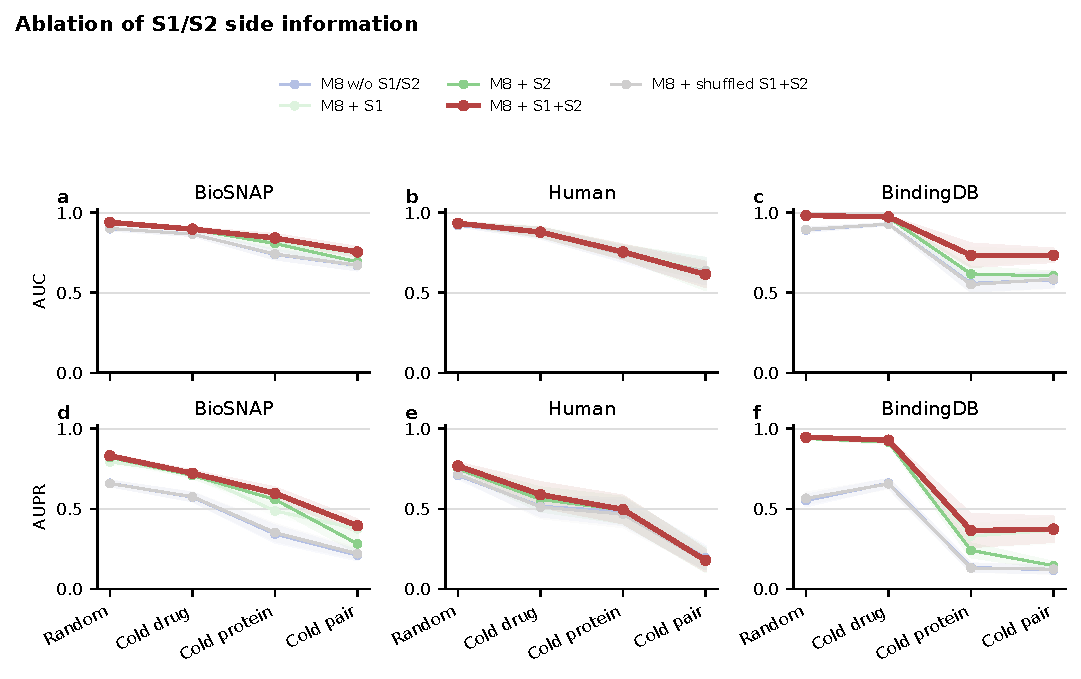
\includegraphics[width=\textwidth]{figures/figure_3_ablation.pdf}
\caption{Ablation of S1/S2 side information. The shuffled control preserves the marginal values of the seven descriptors within each partition but disrupts their association with candidate drug--protein pairs. Each point is the mean of 15 seed--fold evaluations and the shaded band denotes the sample standard deviation.}
\label{fig:side-information-ablation}
\end{figure*}

\begin{table*}[t]
\centering
\scriptsize
\resizebox{\textwidth}{!}{%
\begin{tabular}{llccccc}
\toprule
Dataset & Split & M8 w/o S1/S2 & M8 + S1 & M8 + S2 & M8 + S1+S2 & M8 + shuffled S1+S2 \\
\midrule
BioSNAP & Random & 0.659 $\pm$ 0.015 & 0.793 $\pm$ 0.008 & 0.821 $\pm$ 0.008 & 0.831 $\pm$ 0.007 & 0.658 $\pm$ 0.014 \\
BioSNAP & Cold drug & 0.573 $\pm$ 0.024 & 0.721 $\pm$ 0.017 & 0.708 $\pm$ 0.014 & 0.722 $\pm$ 0.015 & 0.575 $\pm$ 0.024 \\
BioSNAP & Cold protein & 0.342 $\pm$ 0.050 & 0.487 $\pm$ 0.027 & 0.558 $\pm$ 0.049 & 0.597 $\pm$ 0.034 & 0.352 $\pm$ 0.051 \\
BioSNAP & Cold pair & 0.210 $\pm$ 0.029 & 0.375 $\pm$ 0.047 & 0.281 $\pm$ 0.052 & 0.394 $\pm$ 0.036 & 0.220 $\pm$ 0.029 \\
\midrule
Human & Random & 0.709 $\pm$ 0.019 & 0.766 $\pm$ 0.015 & 0.749 $\pm$ 0.020 & 0.768 $\pm$ 0.018 & 0.716 $\pm$ 0.017 \\
Human & Cold drug & 0.516 $\pm$ 0.060 & 0.589 $\pm$ 0.072 & 0.558 $\pm$ 0.072 & 0.588 $\pm$ 0.075 & 0.511 $\pm$ 0.066 \\
Human & Cold protein & 0.482 $\pm$ 0.081 & 0.492 $\pm$ 0.088 & 0.492 $\pm$ 0.079 & 0.496 $\pm$ 0.083 & 0.467 $\pm$ 0.079 \\
Human & Cold pair & 0.195 $\pm$ 0.070 & 0.184 $\pm$ 0.058 & 0.180 $\pm$ 0.072 & 0.178 $\pm$ 0.065 & 0.172 $\pm$ 0.047 \\
\midrule
BindingDB & Random & 0.551 $\pm$ 0.033 & 0.941 $\pm$ 0.004 & 0.939 $\pm$ 0.004 & 0.947 $\pm$ 0.003 & 0.565 $\pm$ 0.033 \\
BindingDB & Cold drug & 0.660 $\pm$ 0.023 & 0.928 $\pm$ 0.006 & 0.916 $\pm$ 0.008 & 0.928 $\pm$ 0.007 & 0.656 $\pm$ 0.026 \\
BindingDB & Cold protein & 0.134 $\pm$ 0.023 & 0.330 $\pm$ 0.070 & 0.240 $\pm$ 0.040 & 0.364 $\pm$ 0.100 & 0.130 $\pm$ 0.021 \\
BindingDB & Cold pair & 0.118 $\pm$ 0.019 & 0.365 $\pm$ 0.078 & 0.145 $\pm$ 0.021 & 0.373 $\pm$ 0.077 & 0.123 $\pm$ 0.026 \\
\bottomrule
\end{tabular}%
}
\caption{Test AUPR for the S1/S2 ablations and shuffled control. Values are mean $\pm$ sample standard deviation across 15 fixed seed--fold evaluations.}
\label{tab:ablation-aupr}
\end{table*}

\subsection{Where the method does not improve}

The complete source data, rather than a selected subset of splits, are used for all comparative statements. In particular, the principal-baseline comparison did not place the full model first in BioSNAP Cold protein, Human Cold protein, Human Cold pair, BindingDB Cold protein, BindingDB Cold pair. These settings are retained in the figures, tables and Discussion rather than being omitted from the main comparison.
